\documentclass[runningheads]{llncs}

\usepackage{graphicx}
\usepackage{enumitem}
\usepackage[utf8x]{inputenc}
\usepackage{comment}
\belowcaptionskip-1em

\begin{document}

\title{LINA: A Serious Game To Help Children With Socialization Problems Using Augmented Reality\thanks{Supported by INESC-ID.}}

\titlerunning{LINA: A Serious Game}
% If the paper title is too long for the running head, you can set
% an abbreviated paper title here

\author{Diogo Filipe Domingos dos Santos Martins - 81983}


%\authorrunning{F. Author et al.}
% First names are abbreviated in the running head.
% If there are more than two authors, 'et al.' is used.

\institute{Orientador: João Miguel de Sousa de Assis Dias \and Departamento de Engenharia Informática \and Instituto Superior Técnico}

\maketitle              % typeset the header of the contribution

\begin{abstract}
To make socialization and interaction with peers easier for children up to pre-adolescence, especially if suffering from a diagnosed social disorder, a game with a strong social component, based on Contact Theory, is proposed. 
\par Using Augmented Reality, the targeted group of children is pitched with finding a missing colleague, searching for clues in a cooperative way, making it necessary to interact with their peers to progress further in the narrative.

\keywords{Augmented Reality \and Contact Theory \and Social Video Game.}
\end{abstract}
%
%
%

\section{INTRODUCTION}

\subsection{Motivation}

\begin{quotation}
"Man is by nature a social animal; an individual who is unsocial naturally and not accidentally is either beneath our notice or more than human. Society is something that precedes the individual. Anyone who either cannot lead the common life or is so self-sufficient as not to need to, and therefore does not partake of society, is either a beast or a god."
\end{quotation}
\par - Aristotle.
\bigskip
\par Nowadays, contact between individuals is increasingly made through digital means: Instant messengers, Voice-over-IP and video calls. Technology allows us to be closer to people, even when they are across the globe. People that do not know each other are brought closer and form social relationships thanks to that same technology. And one particular situation is the approximation of individuals through video games.
\par Quite often the public opinion about video games is slanted towards the negative side, especially among the elderly and/or conservative people, as it was, up until very recently, usually negatively portrayed in the mass media. Indeed, when a mass-shooting occurs and the shooter is a teenager, video games are quickly blamed. However, it is the failure in making the distinction between the various kinds of video games that prevent the public from fully recognizing the potential that video games present as a tool to improve some of society's problems. Even with much of the existing research focusing primarily on violence in video games, gender representation in video games, or using video games for educational purposes, there are some studies that explore the social component of video games and how can players form relationships with each other.


\subsection{Problem}
Socialization is a key process in the psychological development of a child. As the child gradually becomes a teen, his/her \textbf{social cognition} domain starts to expand and his/her awareness towards the social environment around him/her increases steadily. If asked how to describe a friend, that same description changes from physical characteristics and tastes (e.g. "he has brown hair and likes to play football") to more psychological traits, due to him/her starting to perceive the others' actions and behaviours. Also, his/her group of friends shifts from a nebulous semi-structured group of children with whom he/she can have fun and play games to a more heterogeneous and closed group of similar-minded teens that share social activities and opinions (Campos et al. 1990). 
\par As the peer-to-peer relations increase in early pre-adolescence, enthusiast, cooperative and responsive children are usually seen as the more popular in his group of people. However, a child that lacks social interactions, or that feels vulnerable by this psycho-social development and isolates himself, more often will be deem less popular and this can generate anxiety and will diminish the child's self-esteem (Tavares et al. 2007, Campos et al. 1990) creating a snowball into social alienation.
\par So, a child/pre-adolescent that has isolated himself, either by unconscious self-imposition or due to reasons external to him, has diminished social capabilities and lacks will-power and/or opportunities to engage in social activities with others.  \textbf{How can we help improve pre-adolescents' abilities to establish successful relations with their peers?}

%penso que aqui nao devemos restringir o problema a crianas isoladas mas sim a populacao generica. Podes no entanto usar este tipo de crianças como motivacao

\subsection{Hypothesis}

%penso que a tua hipótese está demasiado longa e não é muito clara. Deves focar-te nos aspectos chave: um jogo sério, e contact theory. 
%começa esta secção com os trabalhos que indicam que jogos cooperativos podem ser bons para relações sociais. E depois introduzes a Lina. 

%podes fazer a ponte entre Lina e Contact Theory dizendo que te vais focar nas condições da Contact Theory como por exemplo na "exploitation" de common goals, where users will have to collaborate to discover what happened with Lina.
  
\par There are four concept pillars used to solve the problem described above: Serious Games, Contact Theory, Augmented Reality and User-Centered Design.

\subsubsection{Serious Games}
\par Studies have shown that cooperative video games can bring families closer (Wang, Taylor \& Sun, 2018) and improve the social and affective aspects of hospitalized children by having interactions through a video game context with other children in the same condition (González et al. 2013).  
\par Interestingly, Piper et al. have also explored the possibility of developing social skills in adolescents with Asperger's Syndrome using a cooperative tabletop computer game, which is not far from the project proposed here, and have accomplished successful results with the experiment. However, this project does not need to be restricted to these special circumstances and can be extended to all children in their pre-teens (ages 8-12) as a way to improve socialization, as it was previously shown that prosocial video games can increase prosocial behaviour to all children (Gentile et al. 2009, Griffiths, 2002).

%Studies (Reupert, Mayberry \& Kowalwenko, 2013) have also shown that children whose parents suffered from diagnosed mental pathologies have an increased risk of developing a mental illness themselves, and consequently suffer from decreased interaction with peers due to insufficient socialization skills. 

\subsubsection{LINA}
\par In this document we present a proposal for a serious game, LINA, with a very strong social component. In LINA, a group of players, children from 8/9 to 12 years old, will attempt to find a missing colleague and her story through the discovery of hidden clues, in the form of pictures spread around the school. These pictures will be markers uncovered through augmented reality, sometimes requiring to be uncovered in pairs, which encourages the children to interact amongst themselves to progress further in the narrative.


\subsubsection{Contact Theory}
\par We will be applying Contact Theory when trying to get a group of children to socialize among themselves, thereby trying to improve their relationships, and hopefully creating new ones. In context of the four "positive factors" necessary:
\begin{itemize}
    \item Equal status between groups - All children will have the same importance in the game, all have important information that need to be shared among the others so that they can all advance in the narrative;
    \item Common goals - The shared goal is to finish the game and find what happened to Lina.
    \item Inter-group cooperation - Again, only by sharing the information they have found can they advance in the narrative, so there must be cooperation among themselves.
    \item Support of authorities, law or custom - The teacher, being the authority figure in the classroom, has given the explicit approval and even is directly involved in the game.
\end{itemize}

\subsubsection{Augmented Reality}
\par Augmented Reality is not a new technology employed in the videogame industry, gaining enormous popularity with the worldwide-phenomenon that was \textit{Pokémon Go}. Tateno et al. have inclusively written about the hypothesis that the videogame could help children and teens with severe social withdrawal, although studies were not made to support the claim.
\par The clues about what happened to Lina will be presented in the form of images that can be scanned by a mobile device, and then shown through Augmented Reality.  

\subsubsection{User-Centered Design}
\par As this project will be targeting pre-adolescent children, special care must be considered when designing the concept prototype. A clean, unambiguous interface with established conventions and restricted freedom makes the users' choice-making clearer and and  However, such concept is bound to iterative revisions to improve the users' interaction.

\section{Theorethical Background}

\subsection{Contact Theory}
\par Before Allport hypothesized the "Intergroup Contact Hypothesis" in 1954, it was believed that inter-group contact would inevitably lead to conflict, result from nineteenth century Social Darwinism, where most groups felt superior to others, naturally leading to hostility. However, no studies were conducted at that time and therefore no empirical evidence was found to support the claim. 
\par After the Second World War those suspicions changed. With the desegregation of the United States Merchant Marine in 1948, the relationship between African-American and Caucasian soldiers improved with the number of voyages taken together. Likewise, in a 1957 study by Kephart in the Philadelphia police department, the opinion of white officers regarding fellow black colleagues was more positive in subjects that previously had a black partner.
\par In 1947, Robin Williams Jr., a sociologist in the Cornell University was asked to conduct a review on intergroup relations. On his monograph \textit{The Reduction of Intergroup Tensions} he states that inter-group contact would optimally reduce prejudice under four conditions:
\begin{itemize}
    \item The two groups share similar status, interests and tasks;
    \item The situation fosters personal, intimate intergroup contact;
    \item The participants do not fit in stereotyped conceptions of their groups;
    \item The activities cut across the group lines.
\end{itemize}
\par Allport, in \textit{The Nature of Prejudice (1954)}, after extensive study, would lately adapt these four conditions into four "positive factors" that need to be present to reduce prejudice:

\begin{enumerate}
\item \textbf{Equal status between groups.} This equal status that Allport states refers \textbf{within} the situation, not \textbf{coming into}. Some writers defend that should be of equal status prior to entering the situation, but research has shown that equal status \textit{within} is enough and even more important than outside status.
\item \textbf{Common goals.} To reduce prejudice, active inter-group contact must share a common goal. By having the same objectives, the team constituents work effectively, harder and unitedly, as the different groups rely on each other, to accomplish it.
\item \textbf{Inter-group cooperation.} To work in unity towards the common goal, logically, there must not be group competition. Cooperation should be independently emphasized to each subject, as the feeling of competition undermines the effort made by the rest of the team.
\item \textbf{Support of authorities, law or custom.} With a climate of support surrounding the contact's environment, inter-group contact is more readily accepted and has more positive results. Field research in the military, business and religious institutions has emphasized the importance in support by the authority, as it is that authority that establishes the norms of acceptance.
\end{enumerate}

\par Pettigrew in his revision of the Contact Theory also proposed adding another condition onto the previous set. The condition, \textit{friendship potential} he called it, was a result of his findings where deeply prejudiced groups extremely avoid contact with each other, even when under the four conditions mentioned above. This \textit{friendship potential} condition states that "The contact situation must provide the participants with the opportunity to become friends" (Pettigrew, 1998).


\subsection{Augmented Reality}
\par A variation of Virtual Reality, but different enough to warrant a distinction, the term "Augmented Reality" has been around since the early 1990s, but the whole concept dates back to 1901 when L. Frank Baum in his short story \textit{The Master Key} described a special pair of spectacles that made the person wearing them see a letter on other people's foreheads indicating their personality (e.g. "G" for "good", "E" for "evil", etc). Then in 1968, Sutherland would revolutionize the Virtual Reality topic with the development of a "head-mounted three-dimensional display", and only twelve years later would the first wearable computer, \textit{WireTap}, be invented by Mann, where an optical display would overlay information over the image recorded by a camera. This is a natural evolution of the "heads-up display" used by the military after World War II, where HUDs based in optical reflection presented the information necessary to the pilots without blocking their view in the cockpit.
\par And it is with this last example that the distinction between \textit{Virtual Reality} and \textit{Augmented Reality} become clearer. While the former focuses on creating a separate environment from the user point-of-view, isolating him from his "real" environment, either through visual output, sounds, smells, or even tact, the last tries to enhance the current environment where the user is present, usually capturing it with a camera and overlaying it with information (e.g. text, images) but nevertheless still allowing the user to access the original information captured by his bio-sensors, i.e., eyes, ears, hence "augmenting" his senses.
\par Azuma describes Augmented Reality as systems that:
\begin{itemize}
    \item Combine real and virtual;
    \item Are interactive in real time;
    \item Are registered in 3-D;
\end{itemize}

\par AR has applications in several sectors of society:
\begin{enumerate}
    \item From a medical point-of-view it would be interesting to see and interact with a patient's MRI or CAT scan in real-time; or during a surgery, the surgeon could be accessing in real-time data about the patient or receive feedback about the procedure without having to look away from the operating table.
    \item In engineering, without having to use diagrams nor sketches, if one could see a 3D model of the artifact, the staff training would be rendered much easier. In maintenance, a description of the problem and its solution just from looking to the broken machine would be optimal in keeping minimal downtime and the costs low. 
    \item In the military, pilots have already use the precursor of this technology in their aircraft and more recently have seen it integrated with the helmets and aircraft software, and this also provides a way to soldiers receive real-time information like satellite feeds or drone reconnaissance which helps in reducing the fog-of-war.
\end{enumerate}
And of course, videogames.

\subsection{User-Centered Design}
\par User-Centered Design, is a broad term to describe design processes in which the users affect the development decisions. There are several ways the users can be involved: from requirements gathering and usability testing, to being made partners to designers through the design process.
\par The term User-Centered Design was coined by Donald Norman in his research laboratory in the University of California San Diego, but the concept was formed in his book \textit{The Psychology Of Everyday Things} (1988), where he states four rules for a design to be user-driven:
\begin{itemize}
    \item Make it easy to determine what actions are possible at any moment.
    \item Make things visible, including the conceptual model of the system, alternative actions, and the results of actions. 
    \item Make it easy to evaluate the current state of the system.
    \item Follow natural mappings between intentions and the required actions; between actions and the resulting effect; and between the information that is visible and the interpretation of the system state.
\end{itemize}
\par But just saying a design should be intuitive is not enough, so it is important to considers some additional design principles to facilitate the designer and the user, and which are relevant to this project:
\begin{enumerate}
    \item Simplify the structure of tasks. Make sure not to overload the users' short- and long-term memories. On average the user is able to remember five things at a time. For example, making a long sequence of menus would be counter-productive for a given task. 
    \item Make sure the task in consistent and provide mental aids for easy retrieval of information from long-term memory. Make sure the user has control over the task. In the case of scanning an image and showing a clue the process should be simple and, as it is a frequent action throughout the game, it should not divert from the established loop: \textit{scan, reveal the clue, button to the next stage}. 
    \item Make things visible: bridge the gulfs of Execution and Evaluation. The user should be able to figure out the use of an object by seeing the right buttons or devices for executing an operation. Trying to keep the menus as simple as possible while giving the options necessary, and only those, is a correct implementation of this principle.
\end{enumerate} 
\par As this project is intended to be used by children under 12 years old, special care should be put in place to design a simple, unambiguous, and relatively fun, interface so that it can be easily engaging for the players. 

\newpage
\section{Related Work}

%todas as descrições de trabalhos sobre design e desenvolvimento de jogos devem seguir a mesma estrutura
% Concept, design and development 
% Evaluation, user studies
% Analysis and discussion
% não fales de future work deles. 

\subsection{SIDES: a cooperative tabletop computer game for social skills development (Piper et al. 2006)}

\subsubsection{Concept, design and development}

\par The objective was to develop a cooperative tabletop computer game that encouraged group work skills like negotiation or perspective-taking for students in social group therapy, while taking into account the cognitive strengths and interests of individuals with Asperger's Syndrome.
\par After the interviews made with people suffering from ASD, it was decided to create a puzzle-style game, with a theme of frogs and insects, as its visuals appealed to the interviewed individuals.

\paragraph{Studies and Observations} The authors went to a middle school social therapy class and discussed topics with students and the therapists, trying to understand teaching methods and to identify potential solutions for teaching group work skills. They have also conducted one-on-one interviews with the disorder-affected students but found that group interviews work better. 
\par In terms of results, the students complained about the current group therapy activities, and also gave the suggestion that the game should not appear too "educational", as it would make it uninteresting and not fun. With the therapists, they found that tabletop games were already used as tools during the classes, but close supervision was needed from the therapists as arguments and quarrels were frequent among the students.

\paragraph{Game Rules} The game is played by four players. At the beginning of each round, each player is given nine square tiles with arrows (three of each of three arrow types). Unique arrow types (e.g. pointing left, pointing right, around-the-corner, etc.) are distributed among the participants so that a participant cannot have all 12 arrow types in their hand. Students need to work together to build a path with their pieces to allow the frog to travel from the starting lilypad to the finishing lilypad. There is a limited supply of each arrow type, thus students are encouraged to cooperate in building an optimal path to win more points. To gain points, the path must intersect with the insect pieces on the board, each worth different points. The group must agree on one path that collects the most points with their given amount of resources. Once all players agree with the solution, the frog will travel along the path and collect points by eating all the insects in his way.

\paragraph{Paper Prototype and \textit{DiamondTouch} Implementation} A paper prototype was made to finish the rules, check for game balance and whether the prototype should be turned into a digital game. It was tested with two five-student groups and the feedback was very positive, both from the students and the therapists. The students liked the theme and the game flow was suited. Therapists like how they played cooperatively and had more balanced roles instead of having dominating and least active individuals.
\par After the paper prototype, a digital version implemented in Java for the DiamondTouch multi-user tabletop was made. The players had the same pieces and goal as the paper prototype. Each player had the arrow pieces plus three more \textit{voting buttons}: test the path, reset, or quit the game. This voting system only changes the state of the game if an option is voted unanimously, which gives the players equal status in the situation and forces the group into engaging in communication and coordination.

\begin{figure}
    \centering
    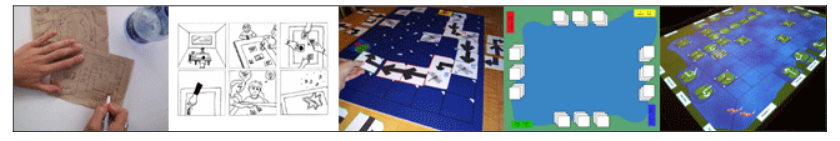
\includegraphics[scale = 0.55]{SIDES.png}
    \caption{The iterative design for this game \textit{(taken from the original article)}.}
    \label{fig:SIDES}
\end{figure}

\subsubsection{Evaluation and User Studies}
\par The first session evaluated if a tabletop game was an appropriate tool for facilitating social skills development and if there was any sensory or motor issues specific to this audience that affected interaction with tabletop technology.
\par The students found SIDES to be a motivating but challenging activity. They also thought the interface was appropriate and easy to use, with much of the excitement revolved around the new technology. There were still some problems regarding the amount of control each player has, with some children pushing each others' hands and shouting, trying to dominate and lead the others.
\par For the next session SIDES was revised: turn-taking and controlled access (i.e. only each player can move their own pieces) were added to prevent other players from interfering with the move, which requires players to communicate and coordinate more.
\par The second session evaluated how students respond to computer- versus human-enforced rules, how the current design aspects encourage or discourage effective group work, and what was the role of the therapist during a tabletop computer activity.
\par Two groups were made: one that had played the previous iteration of the digital game, and another that had only played the paper prototype. They played four rounds each: two with no rules, one with human-enforced rules, which means there was a therapist facilitator, and one with computer-enforced rules.
\par In Group 1, there was an increase in positive language as well as a decrease in the amount of aggressive behaviours over multiple rounds. The computer-enforced scenario was the most well performed, and the no-rules was deemed the worst in terms of team-effort. By the last round, no student touched other players' pieces nor played order-less, having adopted the turn-taking rule naturally.
\par Contrasting to Group 1, Group 2 found the no-rule scenario the easiest of the four to work as a team. Questionnaire data supports this claim, with the rule enforcing being the most disliked. This may be due to a particular individual that would not give up his turn, even when he had no pieces.

\subsubsection{Analysis and Discussion}
\paragraph{Tabletop Technology as a Design Platform} The tabletop provides a place for social interaction, but some students could not reach the other end of the table and the students had to be careful not to misalign the table with the ceiling projector.
\paragraph{Sensory and Motor Issues} The input system was appropriate as all students effectively used the interface and none presented any sensory or motor issue that prevented from playing.
\paragraph{Human- versus Computer-Enforced Rules} The groups in general responded better to computer-enforced rules as it is less subjective than the input from a human, and in their minds, more impersonal and trustworthy.
\paragraph{Embedded Structure} The voting buttons encouraged the users to cooperate and discuss and reach a consensus to progress in the game. Piece ownership balanced the roles of the players by not defining a leader \textit{ab initio}. Computer-enforced turn-taking combined with piece ownership worked for one group but not for the other as mentioned above. In future iterations maybe a hybrid human/computer approach would prevent these situations.
\paragraph{Need for an Adult Moderator} As SIDES was not made as a standalone tool, the presence of the students' therapist is crucial to the experience, as this authority helps them consolidating the abstract topics into shared real experience, and controls the behaviours during the group work sessions.
\paragraph{Challenges in Participatory Design} Due to the special needs of its users, the authors needed extensive preparation in advance, such as lengthy contact with the parents and therapists, encouraging them to participate in the sessions. Sometimes, the students scheduled for an individual interview would "shut down" and no longer answer the questions, which made the authors switch to group interviews.

\bigskip
\par In SIDES, the students made an effort to collaborate and communicate with their peers, which is remarkable as they promptly disengage when unmotivated or uninterested in a task.
\par The authors underline the importance and potential of supportive social entertainment programs through the tabletop technology in dealing with issues amongst a population with special needs. More than that, they stress that the game works because, is not only educational in terms of group work, but also does not appear to be so, which makes it more fun and appealing. Therapists also mentioned how it evens out the class: the more quiet and isolated are "given a louder voice", while the more outspoken and dominating become more restrained in their interventions.



\newpage
\subsection{Pathomon: A Social Augmented Reality Serious Game (Rapp et al. 2018)}

\subsubsection{Concept, design and development}
\par Pathomon takes the premise created by the blockbuster \textit{Pokémon GO} and turns it into a serious game designed to make the players aware of the known viruses and how to eradicate them while being a social experience.

\paragraph{The Story} The player dives into the journey of a young scientist tasked with eradicating viruses.

\paragraph{Game Procedures} Players have to find QR codes, corresponding to antidote ingredients or viruses, in an area. By collecting the ingredients, they can craft antidotes, which then can be used to attack viruses. These actions give the player experience points. Some viruses need to be attacked by more than one player. This, along with having to share the QR codes' locations and the right combination of ingredients to make the antidotes with the other players, gives the game a strong social component.

\paragraph{Mechanics} The player creates a personal account, and then is given a profile of an expert on a certain virus. This means that they can "contaminate" certain QR codes the player has interacted with. This profile also records the player level, his achievements and the global score ladder. The players can level up with the earned experience points, unlocking new viruses and antidotes. The \textit{Pathodex} and \textit{Inventory} records the fought viruses and stores the antidotes, respectively.

\paragraph{Conveying Knowledge} Throughout the game, facts about the viruses are unlocked, like size, lethality, symptoms, incubation time, method of transmission, etc. Some "fun facts" are also stated. Realistic shapes are used for the viruses' appearance in the AR part of the game.

\paragraph{Implementation} The game was made in Unity3D to achieve multi-platform support. For AR, Kudan platform was used. An Amazon AWS EC2 instance attached to an Amazon RDS database hosts the server-side implementation and API. \textit{Pathomon} can be played in iOS and Android devices.

\begin{figure}
    \centering
    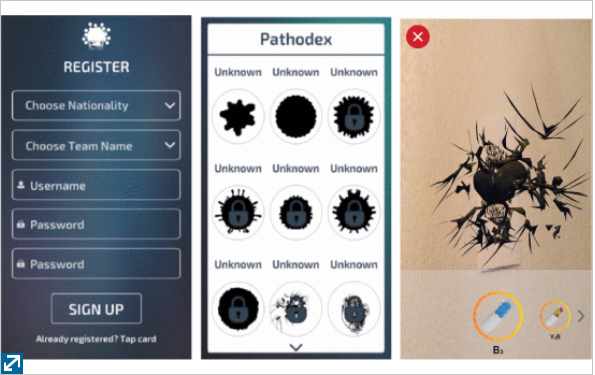
\includegraphics[scale = 0.38]{Pathomon1.png}
    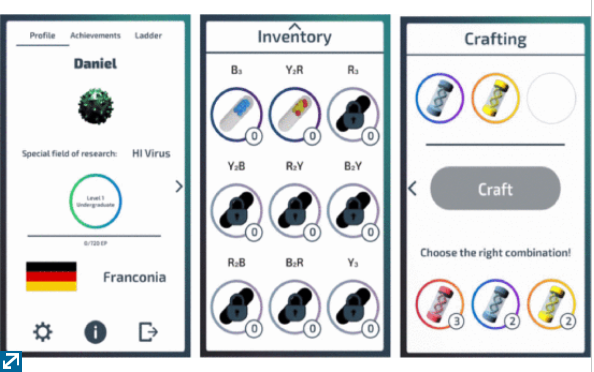
\includegraphics[scale = 0.38]{Pathomon2.png}
    \caption{a) Login, b) Pathodex, c) AR view, d) Profile, e) Inventory, and f) Crafting \textit{(taken from the original article)}.}
    \label{fig:pathomon}
\end{figure}

\subsubsection{Evaluation and User Studies}
\par A study conducted during the 2017 International Genetically Engineered Machine (iGEM) Conference, in which attending people were asked to play the game, revealed that sensory immersion and positive affect were praised, but the game flow and challenge were only reasonable, as they felt the game start and progress too difficult. In the social aspect, the interviewed people did not think their actions could affect the actions of the others, maybe be due to focusing on their own progress. However, this study was made in a poorly controlled environment and with a very low number of subjects, so a follow up study was proposed by the authors to eliminate unreliable results.

\subsubsection{Discussion, Impact \& Conclusion}
\par The user study revealed positive opinions about the game, but still has room for improvement, like the progress and flow. Although the game is used for giving knowledge about viruses, its mechanics could be used in various other contexts.




\subsection{Development of a Videogame to Improve Communication in Children with Autism (Bringas et al. 2016)}

\subsubsection{Concept, design and development}
\par This article refers to the development of a videogame made to improve the communication of children with autism, on the basis that videogames can positively change an ASD-affected child's social behaviour towards other children.

\paragraph{Designing the Content} The authors met with experts on autism to understand what made the children isolate themselves and what techniques and methods were better suited to design an effective tool in complementing the conventional therapy, using the \textit{Theacch, Treatment and Education of Autistic and Related Communication-Handicapped Children}, method.
\par The objective is to improve social interaction by showing a pictogram with basic activities that can be performed in school or at home.
The game's complexity can be changed to adapt to the child's preferences, hence the content shown can change (from a pictogram to images to categories). An important aspect is the positive reinforcement through points and trophies rewarded, promoting motivation to learn and social engagement.

\paragraph{Designing the Game and its Progress} The game design follows the iterative model. Developed in Unity3D for the multi-platform mobile support plus the the ability to be played in a webpage through Unity Web Player.
\par The game takes place in a nature-laden scenery, with the purpose to raise awareness in the child that he is part of an environment and his actions are part of said environment. It focuses on the development of communication and learning abilities through the visual interface and interaction, so that the player feels compelled into finishing all activities within the game.

\paragraph{Description of the Game} The game provides a fun and friendly environment to improve the verbal and non-verbal communication. The game is split into two sections: the \textit{communication panel} and \textit{knowing animals, places and ecosystems}.
\par The communication section shows a thematic panel related with the place or activity. The interface is composed of a group of pictograms of basic activities that can be performed at home or in school. The game allows to eliminate or add images to customize the panel to each individual according to his needs. Through this panel the child can associate meanings to each image, allowing him to express his thoughts and emotions. In the bottom portion of the screen there is a board where he can construct a phrase through the combination of pictures.
\par The \textit{knowing animals} section is made of two modes: Learn and Play. In \textit{Learn Mode} several animals are shown through a name, a real-life picture, a caricature, and with the click of a button, the sound they make.In \textit{Play Mode} the child demonstrates his knowledge about the animals from the previous mode. The picture and caricature of a randomly selected animal appears, and from three different options its name must be chosen. In case of answering incorrectly the game gives another chance, hence the child always ends up choosing the right answer. Upon choosing the right answer points are awarded.

\subsubsection{Discussion, Impact \& Conclusion}
\par Videogames have been shown as successful tools for learning, both technical and social skills. The developed videogame has been positively evaluated by therapists and experts in autistic disorders, and interest has been shown by ASD-affected children, but no studies were conducted.


\begin{figure}
    \centering
    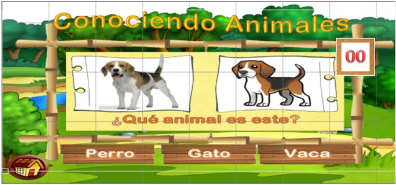
\includegraphics[scale = 0.57]{AnimalArticle1.png}
    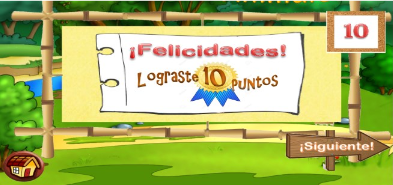
\includegraphics[scale = 0.57]{AnimalArticle2.png}
    \caption{a) Play Mode interface, and b) Achievement Accomplished interface \textit{(taken from the original article).}}
    \label{fig:seriousgame}
\end{figure}


\subsection{Robotic gaming companion to facilitate social interaction among children (Hirose et al. 2014)}

\subsubsection{Concept, design and development}
\par By using a robot that displays human actions like cheering and crying when playing a videogame, this article suggests that children can improve their interaction with robots and humans alike.

\par Problems in socializing have been proven to be reduced through rehabilitation of human-to-human interaction, and one of the approaches used in literature is through a robot, like Kojima's Keepon to encourage interaction in autistic children, as they show an interest towards robots that is not shown towards people.
\par A novel human-robot interaction approach is proposed, to encourage interaction, with the children playing videogames with a robot, but first is necessary to know how can a robotic gaming companion facilitate human-robot and human-human interactions?
\par Videogames are a common medium through which children communicate, plus is fun and engaging. The authors believe that a robotic companion can act as a facilitator in interaction among children playing videogames.

\begin{figure}
    \centering
    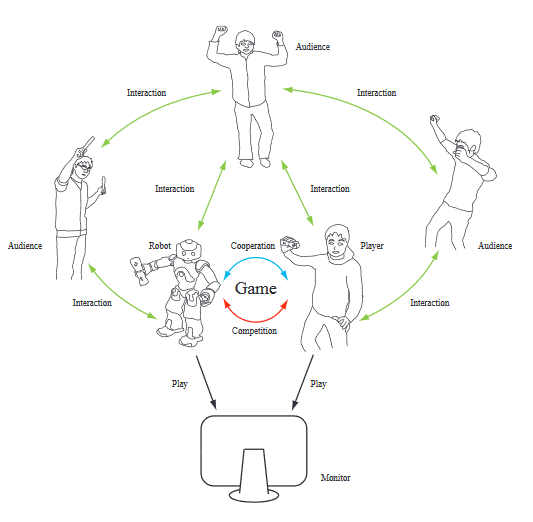
\includegraphics[scale = 0.85]{Robot.png}
    \caption{Gaming communication between the various participants \textit{(taken from the original article).}}
    \label{fig:robot}
\end{figure}

\paragraph{Approach} Communication during gaming can be seen from several perspectives: as cooperative or competitive among players, as between players and audience, and occurring before, during and after gaming.
\par A robot that is able of playing videogames like a human is expected to communicate with those humans. Hence, two factors are studied: playability, i.e. the ability to retain people's attention without natural expressions, and communicability, i.e. the ability to encourage interaction without unnatural expressions. Previous studies stated unnatural expressions should be removed from gaming communication as it affects people's behaviour and ruins the benefits of gaming.
\par The robot must be humanoid and perform similarly to, if not better than, a human, such as it presents a challenge but does not lead to player frustration, nor boredom.

\paragraph{System Overview} Aldebaran Robotics humanoid robot \textit{NAO} was chosen to play Wii videogames (chosen for their strong familiar and social component, bigger than most games in the industry), in particular \textit{Taiko no Tatsujin}, a music video game where the objective is to hit a drum-like controller in the rim or at the center synchronized with the song playing. Score is given by how closely the hits were with the symbols on-screen, much like \textit{Guitar Hero} or \textit{Band Hero}.

\paragraph{Methodology} The game sends an HDMI signal that is split into a computer and a monitor. The signal sent to the computer is then processed and the resulting action sent to the robot. The robot is controlled by two methods: autonomous game play and the Wizard of Oz framework, the last for a smooth and natural interaction with humans.
\par For the autonomous game play, the image received is processed for locating the colors associated with the symbols (red for the center, blue for the rim, orange for the face repeatedly) and calculates the distance and temporal difference from the image's edge until the hit mark, so that calculations are made to know precisely when to hit the \textit{taiko} according to the song's beats per minute.
\par In the WOZ Framework, a doll-type interface was used to wirelessly control the entire body in real time. This allows the user to control the robot by changing the doll's posture. High-level commands like sitting and greeting can be stored and triggered with buttons.

\paragraph{Interaction Scenarios} The robot is capable of three types of interaction: greeting, expression and facilitation. The greeting is executed verbally with a "hello", for example. Expression behaviour are for after gaming, like a "Banzai" when it wins a game, or "Anger" for when it loses. Facilitation is used when cheering for a player or booing an opponent.
\par There are three phases for the interaction: preparation, game and expression. First, in preparation, the robot is assigned as a player or an audience member. As such it performs the appropriate behavior like a handshake or a greeting. In the game phase, it either cheers for a player, or plays the game. In the expression phase, according to the result, the robot shows its feelings, such as "win pose" or "crying".


\subsubsection{Evaluation and User Studies}
\par First an experiment was conducted to see if the robot's performance in-game was similar to a human. After a successful result, a study with children was conducted. The doll operator was out of the child's sight. The robot performed the greeting motion when the participant entered by saying hello, gazing at him, and encouraging him to play the game. During the game phase the robot played autonomously. In the third phase the robot performed their positive or negative behaviour according to the result.
\par The participant's behaviour throughout the experiment was analyzed and found that during the game his interactions rarely occurred during the game phase, perhaps due to be concentrated in the game. However, during the preparation and expression phases the social interactions were recurring.

\subsubsection{Discussion, Impact \& Conclusion}
\par A robotic gaming companion was proposed, with focus on communication, as well as an interaction scenario to ease social interaction among people. In the conducted study the robot introduced has shown that was able to play like a human, and that it was capable of playing a videogame with children and facilitate human interaction.


\subsection{Implementation of an chatbot in a serious game associated with the acquisition of social skills and the promotion of collaborative tasks in children (Mansilla et al. 2017)}

\subsubsection{Concept, design and development}
\par Mansilla et al. propose a serious game as a suplement to therapy in children with emotional disorders.
\par When a child's character is formed, any situation that affects him emotionally in that period will leave him marked in adulthood, hence it is important to care about the child's emotions in this phase. A Serious Game provides the appropriate tool for the necessary therapeutic support.
\par With the game the authors expect to help to overcome moods of sadness or depression, using psychological tools like music therapy and appropriate color management.

\begin{figure}
    \centering
    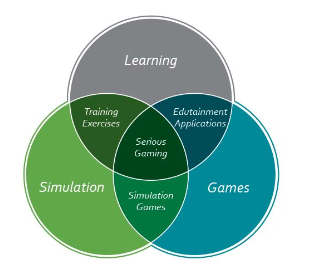
\includegraphics[scale = 0.8]{Chatbot.png}
    \caption{Elements of a Serious Game \textit{(taken from the original article).}}
    \label{fig:Chatbot}
\end{figure}

\paragraph{Prototype Proposed} The prototype will try to counteract the negative emotions present in the child, not engage with the causes responsible for them, through fun and animated scenarios with carefully chosen colors, stimulating his brain through the psychological effects of color. Dark colors are avoided but not completely absent from the prototype.
\par The background music, similarly to colors, will be suited to stimulate the brain through joyful rhythms to lift the spirit.
\par To motivate the child and avoid the feeling of frustration, in case of a low score when finishing the challenge he has the opportunity to repeat it. 
\par There are five scenarios: jungle, sea, desert, polar and forest. First the player registers his name, then selects a difficulty level, from simple to complex. In the simple level the player must choose animals that fit in that scenario and populate it. Every time the player accomplishes an objective triumphant sounds are triggered so that the player's mood can improve. Medals and trophies are also awarded to help with the sense of achievement.
\par Challenges have to be specially considered, they need to be balanced to avoid bringing the player into boredom or on the other hand, into frustration. So, to adapt the challenge's complexity to the player, the combined response of the player's time with his number of hits is calculated. If the player takes too long to rightly place the animals, aiding tracks will be shown to assist him. If the player is rapidly completing the stage then the difficulty increases in two ways: the game gives less time to populate the scenario, or shows animals that are not obvious or well-known.

\subsubsection{Discussion, Impact \& Conclusion}
\par The fact that this project relies on the children emotional support creates an intrinsic complexity. A negative event in such a vulnerable stage can leave the child marked permanently, so this makes it an area of opportunity for research that carries a great impact in personal development. Serious Games presents itself, naturally bridging the acceptance from children and technology as a tool, to improve this problem.



\begin{comment}
\subsection{Design Pattern Canvas: Towards Co-Creation of Unified Serious Game Design Patterns (Zavcer et al. 2014)}

\subsubsection{Concept, design and development}
\par Motivated by the lack of a standardized approach on designing serious games, this article proposes an alpha version based on Osterwalder's Business Model Canvas.

\paragraph{What Are Game Design Patterns?} A design pattern is a solution that can be reused to solve recurring problems, and is described as causes and effects to reach an objective. Not all design aspects are problem solving, especially in game design.
\paragraph{Why Use Patterns for Serious Games Design?} Game design patterns are useful for problem-solving during development as a creative design tool and communication facilitator between peers and professions. Patterns also help to better understand game features and can be used to evaluate design problems, especially in experimental game design.
\paragraph{Criticism of Patterns} Usually patterns are criticized as either too formal or not formal enough, not only in game design, but also in other fields. However, the criticism draws from the quality of their conceptualization, rather than the notion itself, and the fact that patterns are only useful for solving specific problems within the application development.

\begin{figure}
    \centering
    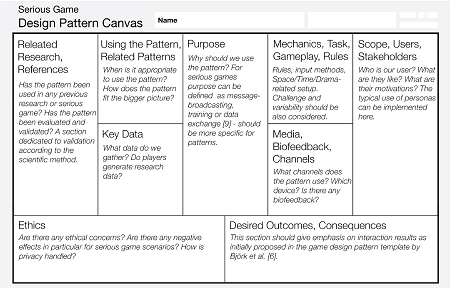
\includegraphics{Screenshot_20.png}
    \caption{Design Pattern Canvas \textit{(taken from the original article)}.}
    \label{fig:DPC}
\end{figure}

\paragraph{Design Pattern Canvas} There are a set of considerations when designing the canvas as to not sacrifice freedom and creativity when designing the experimental prototype. As such the canvas should be:
\begin{itemize}
    \item Intuitive and familiar;
    \item Easy to update and enabling iterations;
    \item Not time consuming to create;
    \item Short (preferably fit on a single page);
    \item Using a widely shared design language;
    \item Facilitating knowledge sharing and transfer;
    \item A Tool to build experimental prototypes directly from the definition of a set of game characteristics;
    \item Standardized;
    \item Considering the perspectives of designer and player;
\end{itemize}

The Design Pattern Canvas (fig.\ref{fig:DPC}) helps to break larger problems into smaller ones and assists in a bottom up approach in designing serious games.
\par The descriptions are not supposed to contain all the information and should be complemented with diagrams. The chart can be split into two sections: the left is associated with design questions and the right is focused on interaction design.

\subsubsection{Discussion, Impact \& Conclusion}
\par The Design Pattern Canvas is a useful tool when designing LINA, 
\begin{itemize}
    \item Related Research, References
    \item Related Patterns
    \item Ethics
    \item Purpose
    \item Key Data
    \item Mechanics, Task, Gameplay, Rules
    \item Media, Biofeedback, Channels
    \item Scope, Users, Stakeholders
    \item Desired Outcomes, Consequences
\end{itemize} 
\end{comment}



\subsection{An adoption framework for mobile augmented reality games: The case of Pokémon Go (Rauschnabel et al. 2017)}

\subsubsection{Concept, design and development}
\par Augmented Reality have recently entered the market and provide the perfect opportunity to bridge the real world with the virtual world, and has the potential to become the next big disruptive market. Pokémon GO is seen as one of those disruptive games, harnessing a large amount of players in a relatively short time span. Existing research focuses primarily in the physical activity undertaken by the users, and miss the why and how consumers play AR games. Also, established theories in existing technology do not consider AR-specific factors.
\par There is also little research on business models for AR games, like the \textit{freemium} pricing used in Pokémon GO, nor take into account the risks players take in their decision-making, so understanding what the underlying psychological mechanisms that drive consumers also improves the knowledge about AR games. So this study seeks to answer what factors drive the gamers' intention to play AR games.

\paragraph{AR versus virtual reality} Research in AR has grown in the last few years, with literature focusing on user adoption behaviour, marketing potential and user requirements. These studies conclude that often the novelty factor drive consumer behaviour, but different factors drive different usage patterns.
\paragraph{Related research} When Pokémon GO launched, it received mixed reviews, praising the physical activity but criticizing it as accident-prone. Limited research exist on the consumers' reaction to mobile AR games and Pokémon GO in particular, showing that a sense of community has been found to be existent within the context of this game, but nostalgia being the most common perceived driving factor. However some unanswered questions remain, as those previous studies focus on the identification of motives, the focus of this study is on the
relationship between gratifications, risks, norms, and different usage patterns.
\paragraph{Uses and gratification theory} This theory addresses why people use a particular media, as it proposes that audiences are goal-oriented and actively select media that can satisfy their individual needs. These needs can be split into five categories:
\begin{itemize}
    \item Cognitive needs: the increasing of one's understanding about a particular issue;
    \item Social integrative needs: the idea that media can help people create new or maintain existing relationships;
    \item Tension-release needs: encompasses aspects such as escapism or diversion;
    \item Affective needs: all forms of emotions, pleasure and moods people want to obtain;
    \item Personal integrative needs: the idea that people engage in certain media to reaffirm their social status or to gain credibility among others. 
\end{itemize}


\paragraph{Model Overview} The authors propose an expanded model of \textit{Uses \& Gratification Theory}, which states that users' evaluation and perceptions of benefits, risks and social influences determine their reactions and intended behaviours. As AR games are hedonistic media, it is proposed that the aforementioned, except cognitive, needs are relevant for explaining benefits brought by them.

\begin{figure}
    \centering
    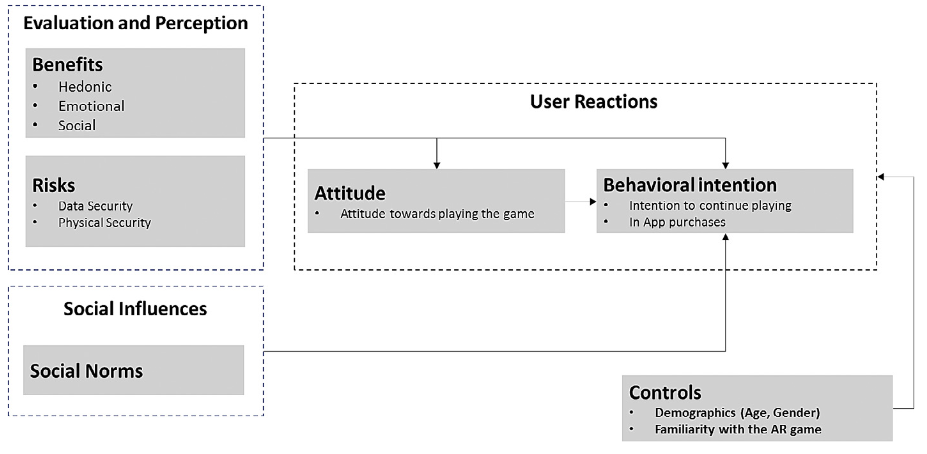
\includegraphics[width=\textwidth]{Screenshot_23.png}
    \caption{Conceptual Model (Overview) \textit{(taken from the original article)}.}
    \label{fig:model}
\end{figure}


\subsubsection{Evaluation and User Studies}
\par A survey to 642 individuals that installed Pokémon GO was made to analyze the proposed model. Pokémon GO was chosen as a study context for being one of the most prominent examples of AR games.
\par The following is a list of hypotheses that were supported in the conducted study:
\begin{enumerate}
    \item Enjoyment, Nostalgia and Physical Activity have a positive effect on users' attitudes toward playing mobile AR games.
    \item Image and Flow has a positive effect on users' attitudes toward playing mobile AR games, and their intentions to continue playing mobile AR games.
    \item Social norms have a positive effect on users' intentions to continue playing mobile AR games.
    \item Physical risk has a negative effect on users' attitudes toward playing mobile AR games.
    \item Users' positive attitudes toward mobile AR games have a positive effect on their intention to continue playing.
\end{enumerate}

\subsubsection{Discussion, Impact \& Conclusion}
\par This study is one of the first attempts to investigate the techniques used that can explain the popularity of mobile Augmented Reality games. In the conducted study it is shown that consumers' attitudes toward playing mobile AR videogames are mostly driven by the level of enjoyment they receive and the image that playing a particular game conveys to other people. Nostalgia, the flow experience and the physical activity also contributes to a positive remark. However, the risk of being injured decreases this attitude. Surprisingly, despite the social activity being a recurring feature, most players do not make use of the socializing benefits that these games could offer.



\subsection{Narrative Design for Rediscovering Daereungwon: A Location-based Augmented Reality Game (Shin et al. 2017)}

\subsubsection{Concept, design and development}
\par Daereungwon is a historical place in South Korea where 23 tombs are located beneath large mounds, being the most famous and main attraction points Michuwangreung, Hwangnamdaechong, and Cheonmachong. However, Daereungwon fails to convey the stories and cultural heritage through the conventional way, due to all tombs appear identical, the scenery being the same from the entrance to the exit, and all the important relics with the historical context being moved permanently 
off-site, leaving the visit with much room for imagination and making invisible the historical backgrounds and details pertaining to each tomb.
\par The goal of this project is to expand the visitors' experience by giving them an added dimension where they can enjoy a gamified interactive narrative focused on increasing the awareness and understanding of the history and cultural heritage found on site. With that goal, the game is designed as a first-person Role Playing Game centered around three points-of-interest: the Michuwangreung,  Hwangnamdaechong, and Cheonmachong tombs. The game application will run on the visitors' mobile devices, and said visitors just need to read markers installed through the visit route, and augmented content will appear superimposed over the physical space. 
\paragraph{Character and Synopsis} The player takes the role of a scavenger trespassing the forbidden burial grounds of the Silla royalty trying to reach Cheonmachong and steal its treasures. The interface gives a first-person perspective of the objects and difficulty-increasing challenges faced in the three stages corresponding to the three points-of-interest. Along the path players encounter objects and characters that will develop the narrative about the player's goal and the past and present of the site.
\paragraph{Integrating Distinctive Point-of-Interest Features} The three different points-of-interest give different contexts and features in the single game narrative, but their information and related stories can be divided in three categories: if the owner of the tomb has been identified, if the excavation of the tombs and its relics was carried out, and the contextual storytelling elements of each of the tombs.

\paragraph{Narrative Design Framework} The game is built around the Memorable Experience Design Framework (Bulencea \& Egger, 2015), that describes a method of creating concept tourism experiences by combining experience staging devices and game design techniques. According to this framework, positive emotions during an experience are generated when there is a stable oscillation between relaxation and tension. This oscillation is vital for tourists to orient themselves in a ready and receptive mindset. Hence, the game starts with easy challenges and progressively gets more difficult, with smaller, relaxing tasks, and rewards between the main challenges so that players do not lose interest and/or get frustrated.
\par The Interest Curve (Schell, 2008) is also applied with the MED framework as a tool to create the progression pattern, maintaining the player's interest level by fluctuating the intensity in a regular pattern while simultaneously increasing it slightly, culminating with the most intense moment in the end, creating an upward curve overall.

\begin{figure}
    \centering
    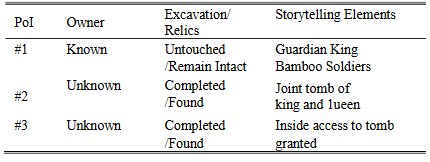
\includegraphics[scale = 0.50]{PoIs.png}
    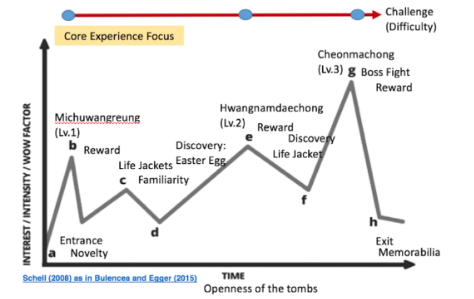
\includegraphics[scale = 0.50]{Schell.png}
    \caption{a) Features of the 3 points-of-interest; b) The game narrative combining elements of the MED framework and the Interest Curve \textit{(taken from the original article).}}
    \label{fig:POI}
\end{figure}

\paragraph{Game Level Design on Each Point-of-Interest} In the first Point-of-Interest, Michuwangreung, bamboo leaves start clouding the augmented interface when the markers are detected and the game starts, with the player unable to proceed further. The leaves transform themselves into soldiers, and the player must "push away" all these soldiers out of the augmented screen by hitting them from the biggest to smallest. When the player accomplishes the mission, the screen is cleared of the bamboo soldiers/leaves and a virtual gate augmented over the real gate opens, and he gets a shovel.
\par In Hwangnamdaechong, the second Point-of-Interest, an animation showing the once separate 
tombs joining one another over the real tomb is augmented on the screen once the marker is detected. The challenge here is to shovel in as many of the queen’s treasures that are flying out of the tomb with the shovel given in the first stage, hence, it is impossible to play this stage 
without having played the first. The treasures shoveled are transformed into gold coins and, in the end, a map showing the path to the final destination appears on screen.
\par In the last Point-of-Interest, Cheonmachong, Cheonma, the white eight-legged horse, appears at the entrance as the player approaches. Then the player needs to win the battle against Cheonma within a time limit, to gain the Gold Crown and Cheonmado (ancient treasures). The gold coins previously earned can be used to purchase weapons and armor, making it easier to play this stage if played the previous ones. Once the player exits Daereungwon after accomplishing the challenges, all the treasures disappear from the game application. 


\subsubsection{Discussion, Impact \& Conclusion}
\par This project uses the Memorable Experience Design framework and Schell's Interest Curve to create an engaging First-Person Role Playing Game experience for the visitors of Daereungwon, in an attempt to convey the cultural and historical heritage that otherwise would not be so thrilling and extensive. 
\par The single cohesive narrative constructed linking the three points-of-interest that fluctuates its intensity while winding up to the climax is the biggest key point here, and seems interesting and relevant to the construction of a similar fluctuating narrative in LINA. 


\newpage
\section{Implementation}

\subsection{Game Overview}
\par Lina, your colleague and friend, did not appear today in class and your teacher knows that she will not come to school anymore, but does not know why. Although she sees your messages, does not answer them, she just sends an enigmatic image and its location. What could that mean?
\par With the first paragraph as premise, LINA is a mobile Augmented Reality in which the student, after a brief introduction exposing the beginning of the narrative with the teacher and the rest of the class (who themselves are also players), goes on searching for the image that Lina "sent" him in the given location. 
\par When scanning an image with the device's camera, an overlayed clue (itself being another image or set of images) is presented, with audio narration exposing a part of the narrative, describing an important event involving Lina, followed with instructions to search for another image. These "stages" are not the same for all players: different players would get different stages so that they would get different pieces of the puzzle. 
\par After completing 1 or 2 "stages", player "A" must find another, player "B", and answer a question related with the story presented to player "B", and vice-versa, forcing the players to interact, share the stories presented to each other, and discussing them. This way the game creates an interesting way of socializing while at the same time exploring a narrative that relates to social isolation. This narrative was designed with the help of a playwright that supplied a script with the introduction dialogue, the narrations, and some initial stages/clues to be implemented in this proof-of-concept. 
\par Also, as a way of rewarding and stimulating the players, achievements and awards will be implemented, as difficulty in the game relates to the location of the image and how challenging the player finds to socialize with others. 

\begin{figure}
    \centering
    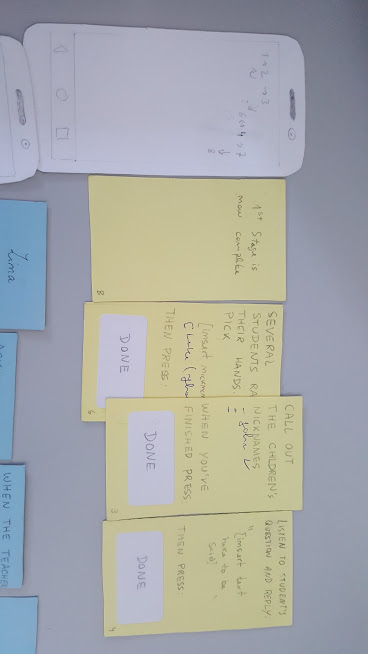
\includegraphics[scale = 0.38, angle = 90]{paper_proto1.jpg}
    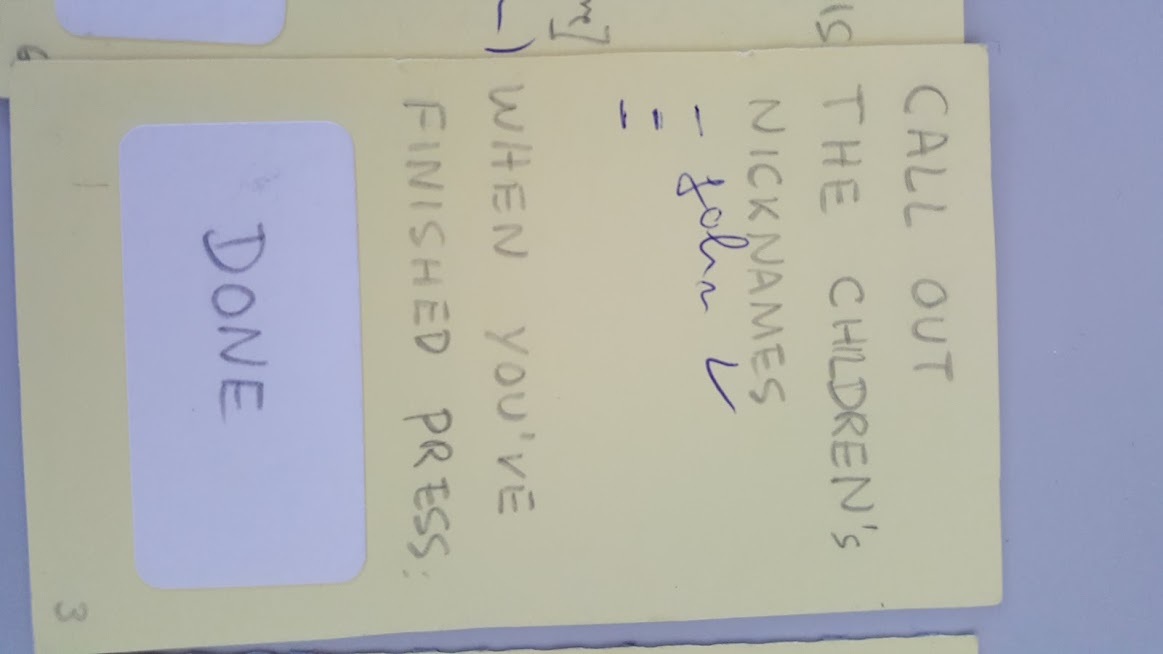
\includegraphics[scale = 0.12, angle = 90]{paper_proto3.jpg}
    \caption{Low-Fidelity Prototype of the teacher's screen.}
    \label{fig:LFP}
\end{figure}

\subsection{Paper Prototype}
\par An initial low-fidelity paper prototype was developed to conceptualize the interface and give some rough guidelines to fulfill the given script. A revision was made after presenting it to specialists and the playwright where some suggestions regarding the presentation of some information texts and buttons. 
\par The interface was chosen to be a simple area of text with some buttons on the bottom of the "screen" (usually "Back" and "Next"), as to keep it simple, so that small children will not be distracted so easily, and to be intuitive, without ambiguities nor entropy. Blue and yellow colors seemed a very pleasant, non-intrusive and neutral background for the players and teacher, respectively.

\begin{figure}
    \centering
    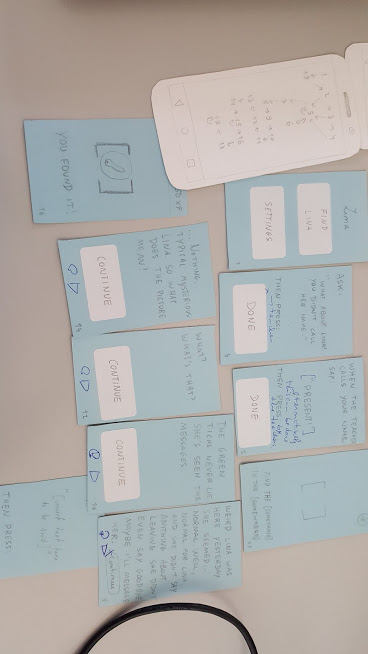
\includegraphics[scale = 0.38, angle = 90]{paper_proto2.jpg}
    
\includegraphics[scale = 0.12, angle = 90]{paper_proto4.jpg}
    \caption{Low-Fidelity Prototype of the children's screen}
    \label{fig:LFP}
\end{figure}

\subsection{Digital Prototype}
\par The digital prototype was made in the Unity3D Engine for its multi-platform support, and the Augmented Reality plug-ins that could be used to implement the scanning part. Initially, we thought that the markers could be QR codes to be scanned, however we decided to go directly for printed pictures instead, as the cost for implementation would be the same and there seemed to be no advantage in starting with QR codes and changing to printed images later on.
\par For the Augmented Reality part we used \textit{Vuforia Augmented Reality SDK}, a plug-in that allows 2D or 3D "markers" to be recognized and overlays an image or object in a position relative to the marker.
\par The game uses a client-server approach to handle communication between the devices, as there must be a server app running serving as game controller. This server also handles the synchronized communication used in the introduction, for example, where a dialogue scene must be coordinated between the teacher and his students. Contrary to the client apps, the server will be run in a computer.

\begin{figure}
    \centering
    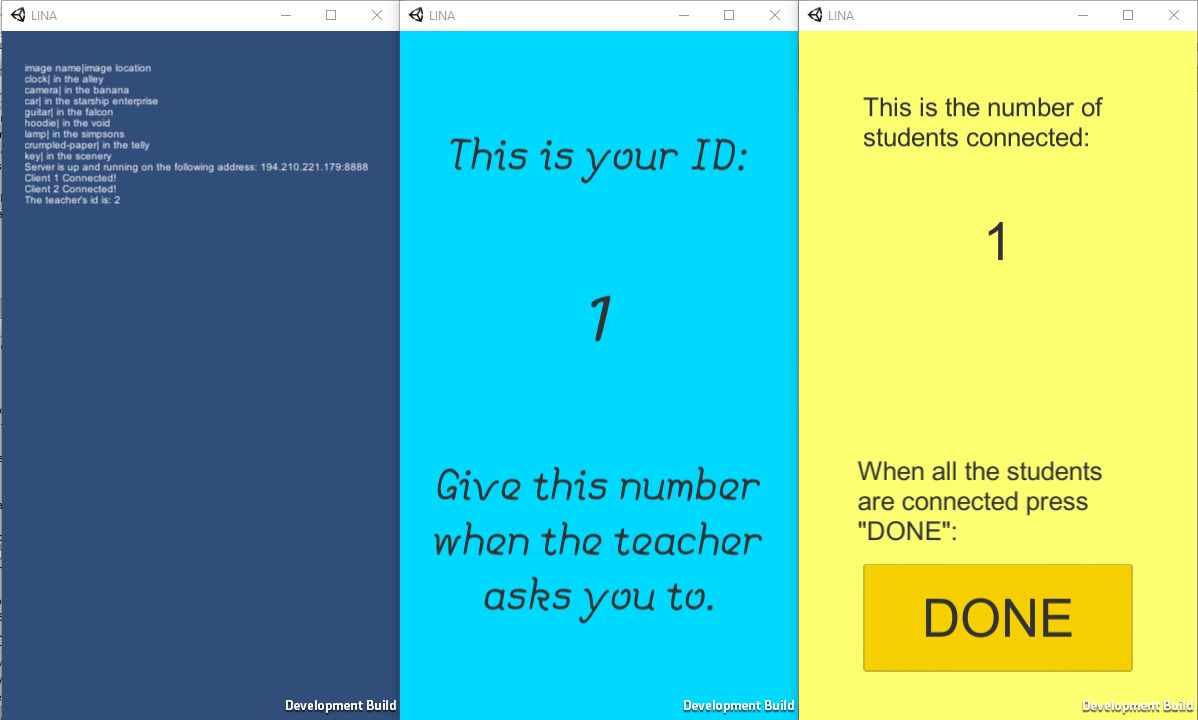
\includegraphics[scale = 0.28]{Screenshot_28.png}
    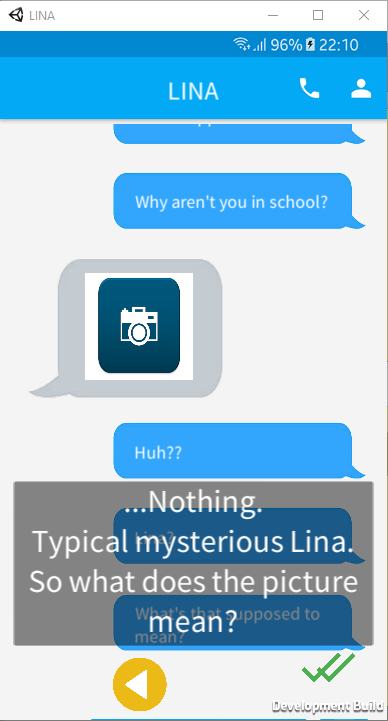
\includegraphics[scale = 0.28]{Screenshot_30.png}
    \caption{These four screenshots were taken from the digital prototype, from left to right: a) The server running in a computer shows the progress of each client similarly to a terminal; b) During the introduction phase, instructions are given to the student on how to interact, similarly to a play; c) The teacher controls the flow of the introduction phase; d) Lina sends a mysterious, and different, image to each player.}
    \label{fig:digital}
\end{figure}

\begin{figure}
    \centering
    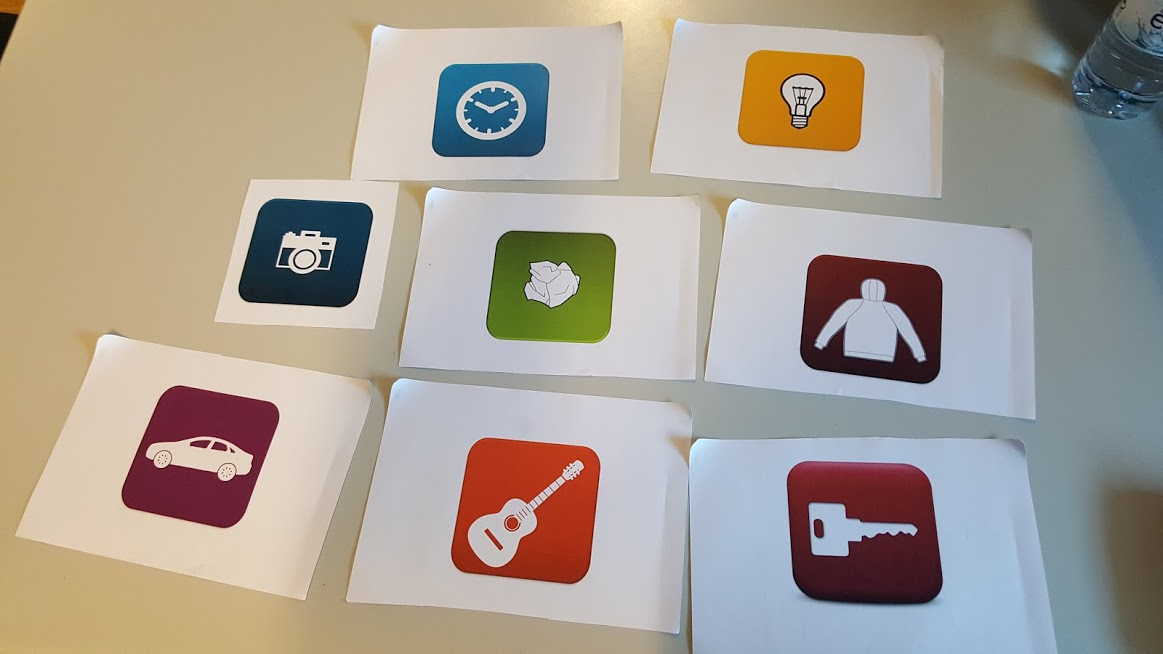
\includegraphics[scale = 0.3]{Icons.jpg}
    \caption{The "clues" that are to be recognized and overlayed through Augmented Reality. These icons were chosen for being images of simple objects that the children could easily recognize. Some are important to the story, like the one with the back of a hoodie sweater. }
    \label{fig:icons}
\end{figure}

\section{Evaluation}
\par To evaluate if this prototype was successful in solving the problem described at the beginning of this document, i.e., in improving the children's relationships with their peers, we need to question them regarding their perceived notion of another person (this "another person" being every other player with whom he shall interact) before and after playing the game. 
\par The \textit{McGill Friendship Questionnaire} is a tool designed to assess friendship in late-adolescents and young adults, however, we do not believe it would be an issue using with pre-adolescents. In this questionnaire, 30 questions regarding how one perceives the other (e.g. "\_\_\_ would be good to have around if I were frightened.", "\_\_\_ would stay my friend even if other people did not like me.") are to be answered in a 9-point Likert scale, which then gives the measurement of several "Friends' Functions": Stimulation Companionship, Help, Intimacy, Reliable Alliance, Self-Validation, and Emotional Security. Through the score in each of these functions it is possible to assess the differences, if any, between the pre- and post-activity. 
\par These results will have to be screened against a control population that instead of playing the game will do another ordinary activity, like a painting exercise or a "normal" class.

%aqui a ideia é descreveres brevemente como é que estás a planear avaliar o teu trabalho de mestrado.

%neste tópico, vais ter de avaliar se o teu trabalho atinge o problema proposto no inicio do documento, ou seja melhorar as relações sociais dos miudos (fazer mais e/ou melhor amigos).

%deves dar ideia do que vais medir (e.g. McGill Friendship Questionnaire), e como vais medir. 

%E.g. Usar uma condição de controle onde os míudos simplesmente fazem uma actividade. Depois tens uma experimental condition onde os miudos usam a Lina, e depois vais fazer pré e pós testes em ambas as condições para determinar se houve um amumento na quantidade e qualidade das relações sociais.

\section{Schedule}

\section{Conclusion} 
\par A game to improve communication between pre-adolescent children using Augmented Reality, and based on Contact Theory, is proposed. LINA provides a cooperative experience where the children search for a missing colleague through clues in the form of augmented images and narrations, superimposed on markers placed around the school. 
\par A low-fidelity prototype was developed, revised by experts and the playwright writing the narrative, and turned into a digital prototype. This solution is evaluated by giving a modified McGill Friendship Questionnaire to be answered by the children after the activity, against a control group.

\newpage
% ---- Bibliography ----
%
% BibTeX users should specify bibliography style 'splncs04'.
% References will then be sorted and formatted in the correct style.
%
% \bibliographystyle{splncs04}
% \bibliography{mybibliography}
%
\begin{thebibliography}{8}

\bibitem{ref_article1}   \textbf{Wang, B., Taylor, L., \& Sun, Q.} (2018). Families that play together stay together: Investigating family bonding through video games. New Media \& Society, 20(11), 4074–4094. \doi{10.1177/1461444818767667}

\bibitem{ref_article2} \textbf{González, C.S., Toledo, P., Collazos, C.A., \& González-Sanchez, J.L.} (2013). Design and analysis of collaborative interactions in social educational videogames. Computers in Human Behavior 31 (2014) 602–611. \doi{10.1016/j.chb.2013.06.039}

%\bibitem{ref_article3} \textbf{Reupert, A.E., Maybery, D.J, \& Kowalenko, N.M.} (2013). Children whose parents have a mental illness: prevalence, need and treatment. Medical Journal of Australia 2013; 199 (3 Suppl): S7-S9. \doi{10.5694/mja11.11200}

\bibitem{ref_proc1} \textbf{Piper, A.M, O'Brien, E., Morris, M.R., \& Winograd, T.} (2006). SIDES: a cooperative tabletop computer game for social skills development. In: Proceedings of the 2006 20th anniversary conference on Computer supported cooperative work, November 04-08, 2006, Banff, Alberta, Canada. \doi{10.1145/1180875.1180877}

\bibitem{ref_article4} \textbf{Gentile, D.A., et al.} (2009) The Effects of Prosocial Video Games on Prosocial Behaviors: International Evidence From Correlational, Longitudinal, and Experimental Studies. Personality and Social Psychology Bulletin, vol. 35, no. 6, June 2009, pp. 752–763. \doi{10.1177/0146167209333045}

\bibitem{ref_article5} \textbf{Griffiths, M.D.} (2002) The educational benefits of videogames. Education and Health, 20(3), 47–51.

\bibitem{ref_book1} \textbf{Campos, B.P., Ribeiro, J.L.P., Fontaine, A.M., Ribeiro, A., Taveira, M.C.} Psicologia do Desenvolvimento e Educação de Jovens vol.II. Universidade Aberta, Lisboa (1990) 

\bibitem{ref_book2} \textbf{Tavares, J., Pereira, A.S., Gomes, A.A., Monteiro, S.M., Gomes, A.} Manual de Psicologia do Desenvolvimento e Aprendizagem. Porto Editora, Porto (2007)

\bibitem{ref_article6} 	\textbf{Tateno, M., Skokauskas, N., Kato, T. A., Teo, A. R., \& Guerrero, A.} (2016) New game software (Pokémon Go) may help youth with severe social withdrawal, hikikomori. Psychiatry research, 246, 848-849. \doi{10.1016/j.psychres.2016.10.038}

\bibitem{ref_article7} \textbf{Kato, T.A., Teo, A.R., Tateno, M., Watabe, M., Kubo, H. \& Kanba, S.} (2017) Can Pokémon GO rescue shut-ins (hikikomori) from their isolated world?. Psychiatry Clin. Neurosci., 71: 75-76. \doi{10.1111/pcn.12481}

\bibitem{ref_article8} \textbf{Pettigrew, T.F.} (1998). INTERGROUP CONTACT THEORY. Annual Review of Psychology, 49(1), 65–85. \doi{10.1146/annurev.psych.49.1.65}

\bibitem{ref_proc2} \textbf{Sutherland, I.E.} (1968). A head-mounted three dimensional display. Proceedings of the December 9-11, 1968, Fall Joint Computer Conference, Part I on - AFIPS ’68 (Fall, Part I). \doi{10.1145/1476589.1476686}

\bibitem{ref_article9} \textbf{Azuma, R.T.} (1997) A Survey of Augmented Reality
Presence: Teleoperators and Virtual Environments 1997 Vol.6, Issue 4, 355-385 \doi{10.1162/pres.1997.6.4.355}

\bibitem{ref_article9} \textbf{Rapp, D., Müller, J., Bucher, K., \& Von Mammen, S.} (2018) Pathomon: A Social Augmented Reality Serious Game, 2018 10th International Conference on Virtual Worlds and Games for Serious Applications (VS-Games), Wurzburg, 2018, pp. 1-4. \doi{10.1109/VS-Games.2018.8493437}

\bibitem{ref_article10} \textbf{Bringas, J.A.S., Léon, M.A.C., Cota, I.E., and Carrillo, A.L.} (2016) Development of a videogame to improve communication in children with autism, 2016 XI Latin American Conference on Learning Objects and Technology, San Carlos, 2016, pp. 1-6. \doi{10.1109/LACLO.2016.7751751}

%\bibitem{ref_article11} \textbf{Zavcer, G., Mayr, S., \& Petta, P.} (2014) Design Pattern Canvas: Towards Co-Creation of Unified Serious Game Design Patterns, 2014 6th International Conference on Games and Virtual Worlds for Serious Applications (VS-GAMES), Valletta, 2014, pp. 1-2.\doi{10.1109/VS-Games.2014.7012153}

%\bibitem{ref_article11} \textbf{Pinto, D., Mosquera, J., Tobar, H., González, C., Fabregat, R., \& Baldiris, S.} (2017) Augmented Reality Board Game for supporting learning and motivation in an indigenous community.

\bibitem{ref_article11} \textbf{ Shin, J., Kim, J., \& Woo, W.} (2017) Narrative design for Rediscovering Daereungwon: A location-based augmented reality game. 2017 IEEE International Conference on Consumer Electronics (ICCE). \doi{10.1109/icce.2017.7889364}

\bibitem{ref_article12} \textbf{Hirose, J., Hirokawa, M., \& Suzuki, K.} (2014) Robotic gaming companion to facilitate social interaction among children, The 23rd IEEE International Symposium on Robot and Human Interactive Communication, Edinburgh, 2014, pp. 63-68. \doi{10.1109/ROMAN.2014.6926231}

\bibitem{ref_article13} \textbf{Mansilla, A., Ochoa, A., Ponce, J., Herrera, M., Hernández, A., \& Cossio, E.} (2017) "Implementation of an chatbot in a serious game associated with the acquisition of social skills and the promotion of collaborative tasks in children," 2017 Twelfth Latin American Conference on Learning Technologies (LACLO), La Plata, 2017, pp. 1-4.
\doi{10.1109/LACLO.2017.8120912}

\bibitem{ref_article14} \textbf{Abras, C., Maloney-Krichmar, D., \& Preece, J.} (2004). User-centered design. Bainbridge, W. Encyclopedia of Human-Computer Interaction. Thousand Oaks: Sage Publications, 37(4), 445-456.

\bibitem{ref_article15} \textbf{Rauschnabel, P. A., Rossmann, A., \& tom Dieck, M. C.} (2017) An adoption framework for mobile augmented reality games: The case of Pokémon Go. Computers in Human Behavior, 76, 276–286. \doi{10.1016/j.chb.2017.07.030}

\bibitem{ref_lncs1} \textbf{Wilkinson, P.} A Brief History of Serious Games. In: Dörner, R., Göbel, S., Kickmeier-Rust, M., Masuch, M., Zweig, K. (eds) Entertainment Computing and Serious Games 2016. Lecture Notes in Computer Science, vol 9970. Springer, Cham. (2016) \doi{10.1007/978-3-319-46152-6\_2}



%\bibitem{ref_lncs0}
%Author, F., Author, S.: Title of a proceedings paper. In: Editor,
%F., Editor, S. (eds.) CONFERENCE 2016, LNCS, vol. 9999, pp. 1--13.
%Springer, Heidelberg (2016). \doi{10.10007/1234567890}

%\bibitem{ref_article0}
%Author, F.: Article title. Journal \textbf{2}(5), 99--110 (2016)

%\bibitem{ref_book0}
%Author, F., Author, S., Author, T.: Book title. 2nd edn. Publisher,
%Location (1999)

%\bibitem{ref_proc0}
%Author, A.-B.: Contribution title. In: 9th International Proceedings
%on Proceedings, pp. 1--2. Publisher, Location (2010)

%\bibitem{ref_url0}
%LNCS Homepage, \url{http://www.springer.com/lncs}. Last accessed 4
%Oct 2017
\end{thebibliography}
\end{document}
